

\documentclass[12pt]{letter}

\usepackage[margin=1in,footskip=0.25in]{geometry}
\usepackage{tikz-cd}
\usetikzlibrary{positioning}

\begin{document}
Class: COMP 3040 - Foundation of Computer Science \\ Name: DangNhi Ngoc Ngo \\ Student ID: 01553277 \\ Homework 1

\centering\textbf{Homework 1: Basics And Using Latex}

\flushleft

\begin{enumerate}
\item[\textbf{0.1}]
\ \\ % create a new line
\begin{enumerate}
	\item A set of all odd natural numbers.

	\item A set of all even integer number.

	\item A set of all even natural numbers.

	\item A set of all even natural numbers that are multiples of 6.

	\item A set of all symmetric binary numbers.

	\item A set of all odd integer numbers.
\end{enumerate}
\ \\ % create a new line
\item[\textbf{0.2}]
\ \\ % create a new line
\begin{enumerate}
	\item \{1, 10, 100\}

	\item \{n $\in$ Z $|$ n $>$ 5\}

	\item \{n $\in$ N $|$ n $<$ 5\}

	\item \{aba\}
	
	\item \{\} or $\varepsilon$

	\item \O
\end{enumerate}
\ \\ % create a new line
\item[\textbf{0.3}] \textbf{Let A be the set \{x,y,z\} and B be the set \{x,y\}.}
\ \\ % create a new line
\begin{enumerate}
	\item \textbf{Is A a subset of B?} \\
				\textit{No. A $\not\subset$ B.}

	\item \textbf{Is B a subset of A?} \\
				\textit{Yes. B $\subset$ A.}

	\item \textbf{What is A $\cup$ B?} \\
				\textit{A $\cup$ B = \{x,y,z\}.}

	\item \textbf{What is A $\cap$ B?} \\
				\textit{A $\cap$ B = \{x,y\}.}

	\item \textbf{What is A $\times$ B?} \\
				\textit{A $\times$ B = \{(x,x), (x,y), (y,x), (y,y), (z,x), (					z,y)\}}
  \item \textbf{What is the power set of B?} \\
				\textit{P(B) = \{\O, \{x\}, \{y\}, \{x,y\}}\}
\end{enumerate}
\ \\ % create a new line
\item[\textbf{0.4}] \textbf{If A has \textit{a} and B has \textit{b} elements, how many elements are in \textit{A $\times$ B}? Explain your answer.}
\ \\ % create a new line
Each element in A is paired with each element in B, so there will be a $\times$ b elements.

\ \\ % create a new line
\item[\textbf{0.5}] \textbf{If \textit{C} is a set with \textit{c} elements, how many elements are in the power set of \textit{C}? Explain your answer.}
\ \\ % create a new line
The power set of \textit{C} $|$P(C)$|$ has 2$^c$ elements. Because the formula to determine a power set is $|$P(C)$|$ = 2$^c$, where C is a set and \textit{c} is a number elements of the set.

\ \\ % create a new line
\item[\textbf{0.6}]
\ \\ % create a new line
\begin{enumerate}
	\item f(2) = 7

	\item Domain f = \{1, 2, 3, 4, 5\} and Range f = \{6,7\}

	\item g(2, 10) = 6

	\item Domain g = \{(x,y) $\in$ N $\times$ N $|$1 $\leq$ x $\leq$ 5, 6 $\leq$ y $\leq$ 10\} \\ Range g = \{6, 7, 8, 9, 10\}

	\item g(4,f(4)) = g(4,7) = 8
\end{enumerate}

\ \\ % create a new line
\item[\textbf{0.7}] \textbf{For each part, give a relation what satisfies the condition.}
\ \\ % create a new line
\begin{enumerate}
	\item \textbf{Reflexive and symmetric but not transitive} \\
				Let R be a set where R = \{(x,x), (y,y), (z,z), (x,y), (y,x), (y,z), (z,y)\} \\
				Reflexive: (x,x), (y,y), (z,z) \\
				Symmetric: (x,y), (y,x), (y,z), (z,y) $\in$ R \\
				Not transitive because (x,y), (y,z) $\in$ R while (x,z) $\notin$ R
	
	\item \textbf{Reflexive and transitive but not symmetric} \\
				Let R be a set, R = \{(x,x), (y,y), (z,z), (x,y), (y,z), (x,z)\} \\
				Reflexive: (x,x), (y,y), (z,z) \\
				Transitive: (x,y), (y,z) $\in$ R and (x,z) $\in$ R \\
				Not symmetric because (x,y) $\in$ R but (y,x) $\notin$ R

	\item \textbf{Symmetric and transitive but not reflexive} \\
				Let R be a set, R = \{(x,y), (y,x), (x,z), (z,x), (y,z), (z,y)\} \\
				Symmetric: (x,y), (y,x), (y,z), (z,y), (x,z), (z,x) $\in$ R \\
				Transitive: (x,y), (y,z) $\in$ R and (x,z) $\in$ R \\
				Not reflexive: (x,x), (y,y), (z,z) $\notin$ R
\end{enumerate}

\newpage
\ \\ % create a new line
\item[\textbf{0.8}] \textbf{Consider the undirected graph G = (V,E) where V, the set of nodes, is \{1, 2, 3, 4\} and E, the set of edges, is \{\{1, 2\}, \{2, 3\}, \{1, 3\}, \{2, 4\}, \{1, 4\}\}. Draw the graph G. What are the degrees of each nodes? Indicate a path from node 3 to node 4 on your drawing of G.}
\ \\ % create a new line
\ \\ % create a new line
(a) Graph G

\centering
\tikzstyle{p} = [draw, circle, minimum size = 1cm]
\begin{tikzpicture}
	\node [p,name =p1] at (0,0) {$1$};
	\node [p](p2) at (4,0) {$2$};
	\node [p,name =p3] at (4,-4) {$3$};
	\node [p,name =p4] at (0,-4) {$4$};
	
\begin{scope}
	\draw (p1) -- (p2);
	\draw (p1) -- (p4);
	\draw (p1) -- (p3);
	\draw [->] (p3) -- (p2);
	\draw [->] (p2) -- (p4);
\end{scope}
\end{tikzpicture}
\flushleft
\ \\ % create a new line
\ \\ % create a new line
(b) Degrees of node \\
Degrees of node 1: deg(1) = 3 \\
Degrees of node 2: deg(2) = 3 \\
Degrees of node 3: deg(3) = 2 \\
Degrees of node 4: deg(4) = 2

\ \\ % create a new line
\item[\textbf{0.9}] \textbf{Write a formal description of the following graph.}
\ \\ % create a new line
\begin{center}
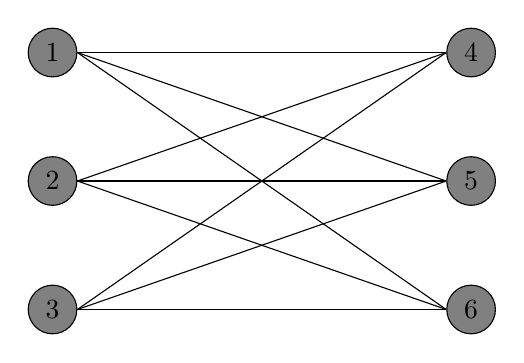
\begin{tikzpicture}[graph/.style={circle, draw, fill=gray}]

\node[graph] (c1) {1};
\node[graph] (c2) [below=of c1] {2};
\node[graph] (c3) [below=of c2] {3};
\node[graph] (c4) [right=5cm] {4};
\node[graph] (c5) [below=of c4] {5};
\node[graph] (c6) [below=of c5] {6};

\draw[-] (c1.east) -- (c4.west);
\draw[-] (c1.east) -- (c5.west);
\draw[-] (c1.east) -- (c6.west);

\draw[-] (c2.east) -- (c4.west);
\draw[-] (c2.east) -- (c5.west);
\draw[-] (c2.east) -- (c6.west);

\draw[-] (c3.east) -- (c4.west);
\draw[-] (c3.east) -- (c5.west);
\draw[-] (c3.east) -- (c6.west);

\end{tikzpicture}
\end{center}

G = (V,E) for any order 

G = \{\{1, 2, 3, 4, 5, 6\},\{(1, 4), (1, 5), (1, 6), (2, 4), (2, 5), (2, 6), (3, 4), (3, 5), (3,6)\}

\end{enumerate}
\end{document} 
